%=========================
% Materials and Methods
%=========================

% 1. What does examination of consequences of networks after imputation mean?
This research mainly examines relationships between the injuries caused by pests and diseases, production situations (e.g., rice variety grown, crop establishment method, fertilizer and chemicals applied), and rice yields using data collected from surveys of irrigated lowland rice growing areas in South and South East Asia. I will develop and apply suitable methods of network analysis to characterize the patterns of co-occurrence of injuries and production situations. The resulting network of associations of injuries and production situations thus provides a starting point for further investigations of their relationships (i.e., comparison of networks from different production environments or examination of consequences of networks after imputation). 

I propose three methods of network analysis using rice crop health survey data. In the following, I present three distinct network analysis approaches: single-network analysis, differential network analysis, and dynamic network analysis. The three approaches answer different questions. 

In the first part of network analysis, I apply single-network analysis in order to defines modules that can then be tested for validity with other data sets. Single-network analysis identifies (a) patterns of interactions (modules) and (b) their key components (e.g., most connected variables) that are present in the data set.

The second part, differential network analysis, I will use to uncover differences in the modules and connectivity between different data sets (e.g., dry season versus wet season). Each data set is then used to construct a network. Next, the networks are contrasted to find (a) non-preserved modules, (b) differentially occurred variables, and (c) differentially connected variables. 


% You're still changing tense. Once I tell you to fix something, please fix it. Do not repeat the mistake. 
% Grammar in last sentence
Dynamic network analysis, in the third part, is applied for studying how networks change at least two different aspects of an evolving complex system. Here I vary yield gains, and obtain data set with different level of yield gains in order to construct a dynamic network of yield varying behaviors. Similar to differential network analysis, dynamic networks focus on comparison of network structure, but it enable us to observe networks changing across successive yield gains. 


\subsection*{Crop Health Survey Data}

The crop health survey data were collected through surveys of farmers' fields in two seasons (wet and dry seasons) from 2009 to 2015 in different production environments across South and South East in irrigated lowland rice growing areas (West Java, Indonesia; Mekong River Delta and Red River Delta, Vietnam; Tamil Nadu and Odisha, India; and Suphanburi, Thailand). The protocol as described by \shortciteA{Savarysurvey2009} was used.

%======= Note ================
% don't leave spaces between letters and punctuation marks, e.g., no space after "(" or before "."
% If you're going to use them, learn the difference between i.e. and e.g. they are not the same
%======================================

% Verb tense, here, still
% See note above for both comments. These still are not fixed here!
% You'd best re-read the protocol to familiarise yourself with just what data is collected and correct what you've written here.
The survey data described above consist of measures of multiple variables with different types of value. Data were divided each sample into three sets of variables, production situation set, injuries and disease set, and yield. \textbf{cropping practice set} are simplified, which collected with many type of data. For example, types of rice varieties (traditional varieties, modern varieties, and hybrid rice), crop establishments ( direct seeded, transplanted rice) were collected in categorical data, pesticide (molluscicide, herbicide, insecticide and fungicide) uses were collected discretized data, and accumulated organic, chemical fertilizers were collected in continuous data. \textbf{Injuries and diseases set} composed of specific signs caused by pests or pathogens (i.e., whitehead, brown spot). They are collected percent of incidence of injury at two rice stages. Two types of injury indices were used areas under progress curves or maximum level of injuries or disease incidence depending on the nature of the injury. The time-dependent information on injuries was thus synthesized and compacted over time.

% 1. If samples composed of incomplete data were removed, why were they encoded in a matrix? sith[clear]
% 2. So you mean complete data? Why are you wording it like this? Awkward.
% 3. Plurality in last sentence.
Samples without incomplete data were encoded as a matrix in which each row represented a surveyed field in a specific location, year and season. Each column represented a collected variables.

\section*{Single Network Development}
% I don't understand the first sentece.
In the case of single network analysis, one use single network for modeling the relationship of cropping practice set, and injuries and disease sets. In the following, I describe a typical single-network analysis for finding the patterns of relationships.
While a single network is the focus, it does not imply that only a single data set is used. Instead, appropriately similar multiple data sets can be used to validate the robustness of module definition and connectivity.

% 1. If I give you comments, I expect them to be addressed, especially simple ones like the following comment here
% 1. (repeated). why do you have "P-values" and "\textit{P} values" are these different P values?
% 2. Punctuation.
In the following, we provide an overview of single-network analysis strategy, which is depicted in Fig. 1: (a) process data preparation, (b) calculate correlation coefficients (Pearson, Spearman, or Kendall). Estimate P-values for all coefficients. Next, determine threshold values for the resulting correlation coefficients and \textit{P} values, storing results in adjacency matrices for the construction of networks, (c) Construct network and analyze network for graph-theoretic properties and infer biological meanings and integrate the network of input data and output data, and (d) yield- related variables are used to prioritize variables within crop health data

\section*{Network of co-occurrence patterns between injuries and diseases}

% introduction
% Verb tense here is changes again? Why?
In the case of single network analysis, I use single network for modeling the pattern of co-occurrence of injuries and disease. In the following, I describe a typical single-network analysis for finding the patterns of relationships. To construct this network, I use survey data selected only the injuries and disease set.

While a single network is the focus, it does not imply that only a single data set is used. Instead, appropriately similar multiple data sets can be used to validate the robustness of module definition and connectivity.

% 1. (repeated). why do you have "P-values" and "\textit{P} values" are these different P values?
% 2. Why is there a " " in yield-related? It's one word. No space.
In the following, I provide an overview of single-network analysis strategy, which is depicted in Fig. 1: (a) process data preparation. (b) Calculate correlation coefficients (Pearson, Spearman, or Kendall). Estimate P-values for all coefficients. Next, determine threshold values for the resulting correlation coefficients and \textit{P} values, storing results in adjacency matrices for the construction of networks. (c) Construct network and analyze network for graph-theoretic properties and infer biological meanings and integrate the network of input data and output data. (d) yield- related variables are used to prioritize variables within crop health data 

% objective
% 1. The rules is to, incorrect grammar
% 2. Capitalization
% 3. Punctuation
This research aims to construct networks visualizing the associations of injuries from pests and diseases with production situations. The rules defining edges of such networks is to present a sufficient level of 'association' between certain attributes of the two nodes. The use of crop health survey data to construct co-occurrence network and perform network decomposition and network analysis has not yet been reported. Additionally, methods performing co-occurrence analysis and co-occurrence networks has not been studied. Thus, evaluation of such methods is challenging because (1) there are many types of variables mixed in crop health survey data. (2) methods can identify variables with true concordance often determine the prior knowledge.(3) methods performing biologically meaningful co-occurrence network construction. 

% The following comment is still not corrected.
% the rules is to present is not grammaticaly correct
This research aims to construct networks visualizing the associations of injuries from pests and diseases with production situations. The rules defining edges of such networks is to present a sufficient level of 'association' between certain attributes of the two nodes. I thus choose correlation measurements to construct an association network based on them.

% methods

\subsection*{\textbf{STEP 1. }\textit{Evaluation of pairwise relationship association methods for network construction}}


% Again, I'm still confused, is this written in past tense (like a normal paper) current (which doesn't make sense) or future (like a proposal should be)? Your verb tenses are not consistent
% Check spelling
% I typically refer to R functions as "function()" to indicate that it is a function, not just a name or a package, e.g. corr.test(), bicor(), etc. You have no standard in your paragraph to identify R functions, that I can see, you use several ways.
% Your last sentence is confusing and incomplete at best, nonsense at worst.

% This whole paragraph needs to be cleaned up, see my comments from previous.

%%% I'm stopping here. You need to spend some time cleaning this section up and making corrections.
To identify the most suitable methods for constructing a network based on correlation measurements, I selected four correlation based measures, Pearson's correlation, Spearman's rank correlation, Kendall's correlation, Biweight midcorrealtion. The cor.test function of R \shortcite{R:2014a} is applied for generating a correlation matrix, which describes the pairwise associations between variable in the context of the crop health survey data. This function allow users to select type of correlation measures to perform such as Pearson's correlation, Spearman's rank correlation and Kandell's rank correlation. "bicor()" function of WGCNA package \shortcite{Langfelder:2008bd} in R is applied for computing biweight midcorrelation matrix. 


% nonsense
\subsection*{\textbf{STEP 2. }\textit{Comparison of threshold selection methods correlation matrix of survey data}} 

% first sentence is nonsense, rewrite
% second sentence is nonsense, rewrite
% consider the purpose of this whole paragraph and write it more clearly.
When a correlation matrix was create, next is to construct the correlation based network from the correlation matrix. However, the matrix is required the removal of spurious relationships by using threshold. Threshold is a value used for screening the correlations, if correlations  below a threshold value, or close to zero, will be less meaningful, then will not be shown in network graphs. Threshold selection is statistically based, which can be obtained in two ways \shortcite{Toubiana:2013cv}(1) Determine \textit{P} values for all pairwise comparison and adjust them for multiple hypotheses testing (e.g., Bonferroni or local false discovery rate. (2) Obtain a threshold value that guarantees a pre-specified false-discovery rate.


% why knowledge of biological literature? Why not a good understanding of the biological system that you are monitoring? I think that's more essential and useful
\subsection*{\textbf{STEP 3. }\textit{Evaluation of the network inference with a good understanding of the biological system or documented biological relationships}} 

% models cannot reveal knowledge, look up the definition of knowledge. It does not apply here. What do you really mean because it can not be knowledge?
Although we can opt for a method based on its principle of statistical operation without paying attention to the biological models in a given data set, this may not lead to a coordination network that will reveal biological knowledge. 

% first sentence, all of them what?
% based on what study? Our study? Who is "we"? This is YOUR research. If anything it should be "based on my study" but I'm not clear as to what study you refer to here. Who are the "we" that are suggesting? You're the only author on this manuscript. It's your disseration. There is no, our, us or we. It's only my, me, I here.
% Is "codes" the proper form to use?


%There is no statistical method that is suitable for all of them. Identification of the most efficient method for knowledge discovery of a specific biological process demands concrete prediagnostic analyses. Based on our study and our empirical knowledge, we would suggest the following procedure for identifying the most appropriate gene association method for a specific biological theme in a given data set: (1) Evaluate the prior knowledge of biological processes of one’s interest, and select a few known genes involved in these processes; (2) Use the R codes from this study to perform a genome-wide coexpression analysis to obtain the top 100 or 500 genes that are most closely associated to the selected known genes; (3) Perform an evaluation of these 100 or 500 genes by examining which methods can associate the more functionally relevant genes to the selected genes. This can be achieved by examining gene annotation or performing GO term enrichment analysis: and (4) Choose the best method for the data. However, if prior knowledge of biological theme of one’s interest is lacking, we suggest the most stable gene association method.
 
%Physical and genetic interaction networks provide key insights into complex biological systems

Injuries and diseases, and production situations interaction networks provide key insight into complex system 

\section*{Differential Network Analysis}  % incomplete

% introduction
Differential networks can be used to describe differences between two networks under different conditions. They might display different interactions that is fundamentally distinct from the original networks. The strongest differential interactions are not necessarily that are strong in static conditions, or they are clearly changing. Conversely, interactions present in both conditions are weak or removed from the differential network. You may infer that if networks constructed from different environment conditions, differential interactions between two networks imply changes that are a result of response to environmental conditions. 

% objective
My objective of differential network analysis is to extract interactions from the static network that appear to be active under different conditions. I focused two aspects of this analysis. The first is for comparison interaction of cropping practices and injury profile network changes across multiple production environments, and second is to study how networks changed under different seasons. 
% methods

Based on the methods of single network construction mentioned above, differential networks were constructed from survey data with different groups of samples following the purpose of network construction. For differential networks at different seasons, I constructed the first network using the dry season and the second network using wet season. 

To compare two networks, I apply WGCNA package in R, which this package provide several function to analyze the   difference of two networks with the instructions from (Book Weight network analysis) For example, \textit{horvath2011weighted} function is used to compare between the connectivity measures of each network. 

%I propose the overview of differential networks are illustrated in Figure \ref{fig:wholenet}.


% why is 2.3 not 2.1? % The problem there is that you must put the label after a caption, so the label can reference to the figure (it references to the caption, actually). See here: http://www.latex-community.org/forum/viewtopic.php?t=3659 I've corrected this. - ahs
 
%We describe another application of WGCNA, differential network analysis, which may be useful in identifying gene pathways distinguishing phenotypically distinct groups of samples. In our example, we identified the 30 mice at both extremes of the weight spectrum in the B · H data and constructed the first network using the 30 leanest mice and the second network using the 30 heaviest mice. For the ith gene, we denote by k1(i) and k2(i) the whole-network connectivity in networks 1 and 2, respectively. To facilitate the comparison between the connectivity measures of each network, we divide each gene connectivity by the maximum network connectivity, i.e.,

\section*{Dynamic Network Analysis} % okay edit one more round for more consistancy
% introduction

Biological systems are highly dynamic that must continuously respond to a external or internal change of the system, or they can be altered more slowly over time, so realistically the corresponding network graphs evolve as well, and should be analyzed. It seems clear that if we are able to develop a complete understanding of biological systems, we must understand the systems on how their dynamic effects are, they are affected by, changes in the different conditions . Some understandings were obtained from studies of dynamics of large networks, for example, gene expression or metabolic fluxes network \shortcite{Idekerdiffnet}.

Dynamic network analysis is applied for study changes of networks at least two different aspects of an evolving complex system. The main goal of this analyais move away from characterizing absolute properties of the system to concentrate on a specific dynamic systems response. Rather than answer what the key factors in the sytem, they answer what parts of the system are most affect by perturbation.

From the context of crop health survey data, yields are affected from dynamic interactions between pests, plants and environments including cropping practices. The results from damages of pests and disease will be able to lead to yield loss. Hypothetically, Different yield gains are the consequence of different patterns of interaction between injuries and disease, and production situations.

My objectives are to construct networks of crop health survey data at different level of farmers' yields. When networks were generate, I will perform dynamic network analysis. This analysis will enable us to find out how network of change when yield gains decreased or increased.


To obtain the data for constructing the dynamic network, I vary yield gains, and obtain different yield data set in order to construct a dynamic network of yield varying behaviors. I employ "networkDynamic" \shortcite {networkdynamicpackage} and "ndtv" \shortcite{ndtvpackage} packages to generate yield-varying networks. The dynamic graphs will be characterized following \shortcite{bilgin2006dynamic, kolaczyk2014statistical}



\subsection*{Analyzing the Structure of Network Models}

% edited for Tex code
Once networks are constructed, several indices can be computed that convey information about network structure. Structural properties of networks can be used for the interpretation of datasets and for generating hypotheses. Two types of structure are important. First, typically one is interested in the global structure of the network (random networks, small networks, scale-free networks) \shortcite{Strogatz:2001wc, Jeger:2007tn}. Second, one may be interested in local patterns, which are characteristics of each node. For example, clustering of nodes and/or edges in a network can identify groups of nodes with similar properties, and these are referred to ``modules'' or ``communities''  \shortcite{osorio2012integrative, Jeger:2007tn}.

% edited for clarity
For deep insights, comparing the networks by using some key topological properties of network are usefully conducted. Degree and degree distribution of a network is a simple property to extract from network models, which are the number of connections of each node and the frequency distribution of the number of connections per node, respectively. Cluster coefficient is the other measure, which is the value that is able to indicate whether the entities in network form cluster or group within network structure. \shortciteA{Deng:2012do, newman2003structure, Toubiana:2013cv} are recommended references for descriptions of the network properties as well as the formal calculation of these measures.


%\begin{landscape}

%\begin{figure}[h!]
%\centering
%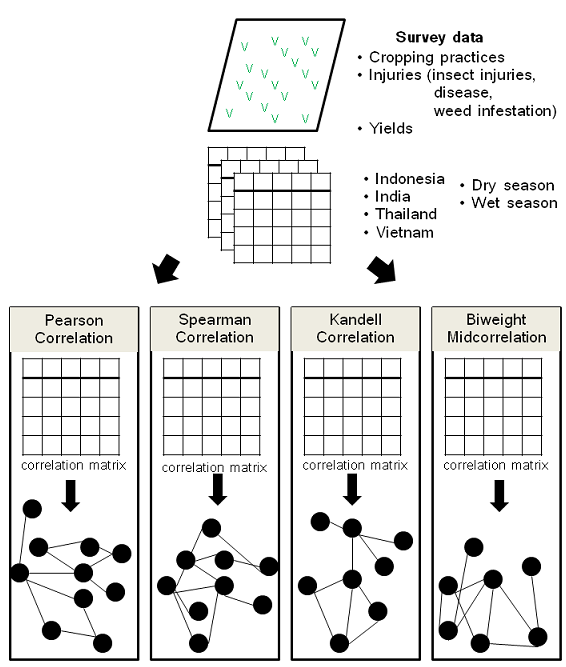
\includegraphics[resolution = 600]{pipeline}
%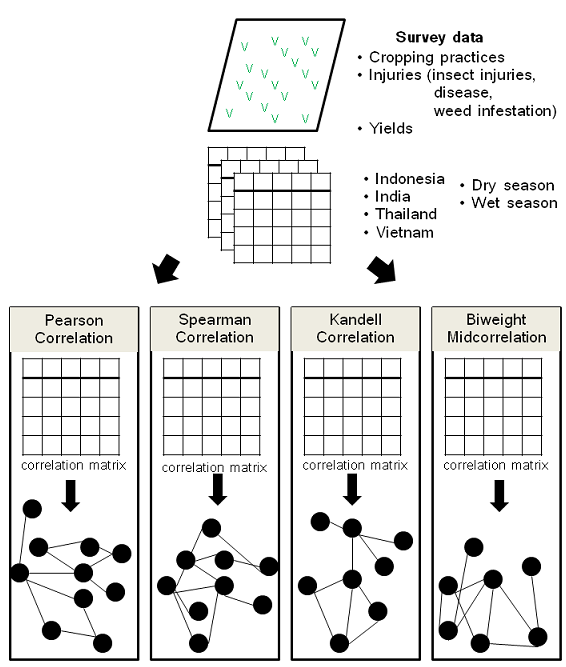
\includegraphics[width=6in]{pipeline}

%\caption[Proposed pipeline for network construction]{Proposed pipeline for network construction. (a) Collect the input profiling data and output profiling data from different samples and different locations. (b) Calculate correlation coefficients (Pearson, Spearman, or Kendall). Estimate P-values for all coefficients. Next, determine threshold values for the resulting correlation coefficients and \textit{P} values, storing results in adjacency matrices for the construction of networks. (c) Construct network and analyze network for graph-theoretic properties and infer biological meanings and integrate the network of input data and output data. (d) Repeat analysis for a second season to verify the network model.}
%\label{fig:pipeline}
%\end{figure}
%\end{landscape}

%\newpage
%\begin{landscape}
%\begin{figure}[h!]
%\centering
%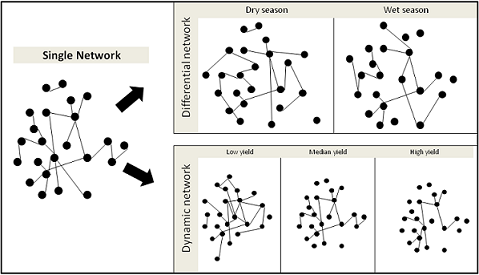
\includegraphics[width=6in]{wholenet}

%\caption[Network comparison]{Network comparison: Network models constructed from survey datasets of different geographic locations are compared by determining their properties. Networks will express the conserved domains within their structure. A merged representation of the two networks being compared is also proposed as a holistic network of rice ecosystem in South and South East Asia.}
%\label{fig:wholenet}
%\end{figure}
%\end{landscape}

%================eos================================

